
\documentclass[12pt,letterpaper]{report}
\usepackage[margin=1in]{geometry}
\usepackage{graphicx}
\usepackage{amsmath}
\usepackage[font=small,labelfont=bf]{caption}
\usepackage[justification=centering]{caption}
\newlength \figwidth
\setlength \figwidth {0.75\linewidth}

\begin{document}

\title{E153 Laboratory Assignment \#1}
\author{Courtney Keeler and Stephen Pinto\\
Harvey Mudd College}
\date{September 30, 2013}
\maketitle

\begin{center}
List of Materials:
\begin{itemize}
	\item Tektronix 2212 Oscilloscope
	\item Hewlett Packard 33120A Function generator
	\item Pomona 4550B (10X probe)
	\item Multimeter
\end{itemize}
\end{center}

\section*{Section A: Analog Oscilloscope vs. Digital Storage Oscilloscope}
\subsection*{Procedure}
\begin{enumerate}
	\item Turn on the Hewlett Packard 33120A Function generator, set the out term to High Z and the amplitude to 1 $\text{V}_{\text{pp}}$
	\item Connect the of the function generator to the channel 1 input of the Tektronix 2212 Oscilloscope with a BNC cable
	\item Turn on digital storing on the oscilloscope (digital)
	\item Set the function generator frequency to 1 Hz and record the amplitude and frequency of the signal displayed by the oscilloscope
	\item Repeat the previous step with frequencies of 1kHz, 1MHz, and 10MHz
	\item Repeat the two previous steps with the oscilloscope's digital storing turned off (analog)
\end{enumerate}
\subsection*{Results}
\begin{table}[ht]
\caption{Presentation of Sin Waves} % title of Table
\centering 
    \begin{tabular}{| c | c | c |}
    \hline  
    Frequency & Analog & Digital \\
    \hline
    1 Hz & * & 283.1 m$\text{V}_{\text{pp}}$, 991.5 mHz \\
    1 kHz & 1.012 $\text{V}_{\text{pp}}$, 1.025 kHz & 1.003 $\text{V}_{\text{pp}}$, 1.002 kHz \\
    1 MHz & 1.003 $\text{V}_{\text{pp}}$, 1.003 MHz & 991.7 m$\text{V}_{\text{pp}}$, 1.00 MHz \\
    10 MHz & 976.2m$\text{V}_{\text{pp}}$, 10.06 MHz & ** \\
    \hline
    \end{tabular}
    \label{table:SinWave}
\end{table}
* Can see the sin wave moving across the screen but cannot capture samples and therefore cannot measure signal

** Can't be measured since time scale minimum is .4us/div while storing is on
\\[.1in]
Table \ref{table:SinWave} shows that the analog scope is favored for high frequency measurements, while the digital scope is favored for low frequency measurements. This is due to the fact that the analog oscilloscope cannot store past values, so at low frequencies, the oscilloscope displays a continuously moving signal. For a higher frequency signal, this is not an issue because the movement of the signal on the screen cannot be perceived by the human eye and appears static (and can therefore be measured). The digital oscilloscope can store past data points and therefore display a measurable signal at very low frequencies. However, the time required to perform an A/D conversion and store the value limits the upper frequency at which the digital oscilloscope can operate. While this setting stills displays data for a 10MHz signal, the user is unable to zoom far enough in on the screen to measure the frequency of the signal seen.

\section*{Section B.1: The 10X Scope Probe}
\subsection*{Procedure}
\begin{enumerate}
	\item Cut two pieces of wire and strip the both ends of each
	\item Insert one end of each wire in each slot of the capacitance measurement slot in the Multimeter
	\item Connect a BNC splitter to one end of a BNC/Coax cable
	\item Connect the positive lead of the splitter to the available end of the wire in the positive capacitance measurement terminal
	\item Repeat the above step for the negative lead and negative terminal
	\item Record the displayed capacitance
	\item Replace the BNC/Coax cable with the Pomona 4550B 10X probe (attaching probe tip to positive terminal and ground clip to negative terminal)
	\item Record the displayed capacitance
\end{enumerate}
\subsection*{Results}
\begin{center}
\begin{table}[ht]
\caption{Capacitance}
\centering
	\begin{tabular}{| c | c |}
	\hline
	
	\textbf{BNC/Coax} & \textbf{10X Probe} \\
	\hline
	108 pF & 21 pF \\

	\hline
	\end{tabular}
\end{table}
\end{center}

\subsection*{Calculations}
The resistive and reactive loading are found by circuit analysis. For the BNC cable, the circuit is shown in Figure \ref{fig:bnc_circuit}.

\begin{figure}
	\centering
	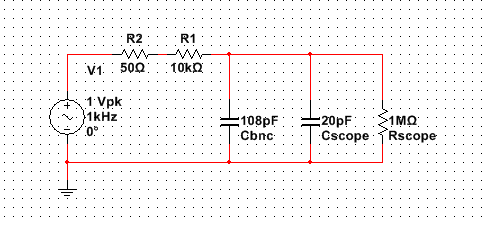
\includegraphics[width=\linewidth, keepaspectratio=true]{lab1_images/BNC_circuit.png} 
	\caption{Circuit model of a BNC cable connecting a function generator (with an additional 10k resistor in between) to an oscilloscope}
	\label{fig:bnc_circuit}
\end{figure}

We can see that the only resistive element is the 1M$\Omega$ resistor, so this resistance value becomes the resistive loading of the circuit. The circuit of the 10X probe is shown in Figure \ref{fig:probe_circuit}.

\begin{figure}
	\centering
	\includegraphics[width=\linewidth, keepaspectratio=true]{lab1_images/10x_circuit.png} 
	\caption{Circuit model of a 10x probe connecting a function generator (with an additional 10k resistor in between) to an oscilloscope}
	\label{fig:probe_circuit}
\end{figure}
 
Here we see that there are two resistive elements in series. The total resistive loading of this circuit becomes the sum of the two resistance values: 10M$\Omega$. These results are summarized in Table \ref{table:ResistiveLoading}.

\begin{center}
\begin{table}[ht]
\caption{Resistive Loading} % title of Table
\centering 
	\begin{tabular}{| c | c |}
	\hline
	
	BNC/Coax & 10X Probe \\
	\hline
	1 M$\Omega $ & 10 M$\Omega$ \\

	\hline
	\end{tabular}
	\label{table:ResistiveLoading}
\end{table}
\end{center}

To calculate the reactive loading of the BNC and 10X probe circuits, we analyze the capacitors only (if these circuits included inductors, they would be analyzed here too). For the BNC model, Figure \ref{fig:bnc_circuit} shows two capacitors in parallel. To find the total reactive loading, we add their values and find the impedance (Z) of the combined capacitance:
$$ \text{C}_{\text{total}} = 108 \text{pF} + 20 \text{pF} = 128 \text{pF} $$
$$ \text{Z} = \frac{1}{\text{j}\omega\text{C}_{\text{total}}} $$
The $\omega$ term refers to signal frequency, and we must evaluate for 100 Hz, 1kHz, and 1MHz. The results are summarized in Table \ref{table:ReactiveLoading}.

For the 10x probe model, Figure \ref{fig:probe_circuit} shows the only reactive elements are three capacitors - one in series with two in parallel. The total capacitance of these three capacitors is
$$ \text{C}_{\text{total}} = \frac{18 \text{pF} (53 \text{pF} + 20 \text{pF})}{18 \text{pF} + 53 \text{pF} + 20 \text{pF}} = 14 \text{pF} $$

 
\begin{center}
\begin{table}[ht]
\caption{Reactive Loading}
\centering
	\begin{tabular}{| c | c | c |}
	\hline	
	Frequency & BNC & 10X Probe \\
	\hline
	100 Hz & 12.4 M$\Omega$ & 110 M$\Omega$\\
	1000 Hz & 1.24 M$\Omega$ & 11.0 M$\Omega$\\
	1 MHz & 1.24 k$\Omega$ & 11.0 k$\Omega$\\	
	\hline
	\end{tabular}
	\label{table:ReactiveLoading}
\end{table}
\end{center}

Note that for the 10x probe, the reactive and resistive loading magnitudes are equivalent at

$$ \frac{1}{2 \pi f\text{C}_{\text{total}}} = 9 M\Omega \Rightarrow f = 1.22 kHz $$.

\section*{Section B.2: The 10X Scope Probe}
\subsection*{Procedure}
\begin{enumerate}
	\item Connect the function generator to the bread board using a BNC cable and splitter
	\item Put a 10k$\Omega$ resisistor in series with the generator output
	\item Connect a BNC cable from the resistor to the oscilloscope
	\item Turn the function generator on and output a sine wave
	\item Increase the frequency until the magnitude measured by the scope is 0.707 times that coming from the function generator (1 $\text{V}_{\text{pp}}$)
	\item Record that frequency (which is the corner frequency)
	\item Repeat the steps 3-5 for a 10x probe
	\item Build the circuit models in ModelSim and run the simulation tool to verify the measured corner frequencies
	\item Use MATLAB to estimate what a square wave and triangle wave would look like through each circuit at the corner frequency and 10x the corner frequency
\end{enumerate}

\subsection*{Measured Results}

\begin{figure}
	\centering
	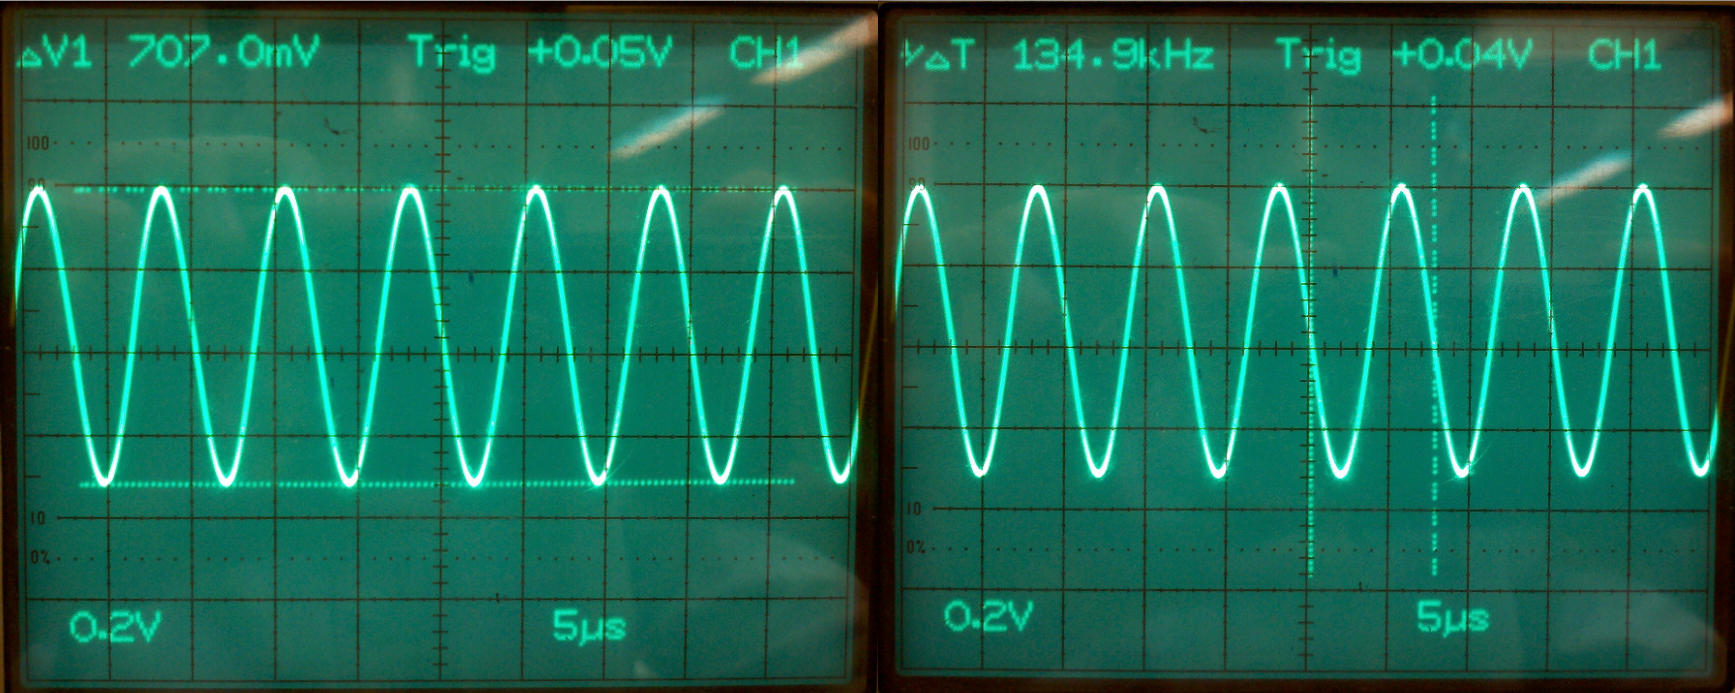
\includegraphics[width=\linewidth, keepaspectratio=true]{lab1_images/BNC_sine_corner.png} 
	\caption{Oscilloscope reading at corner frequency (135 kHz) for BNC cable in series with a 10k resistor. }
	\label{fig:bnc_corner}
\end{figure}

\begin{figure}
	\centering
	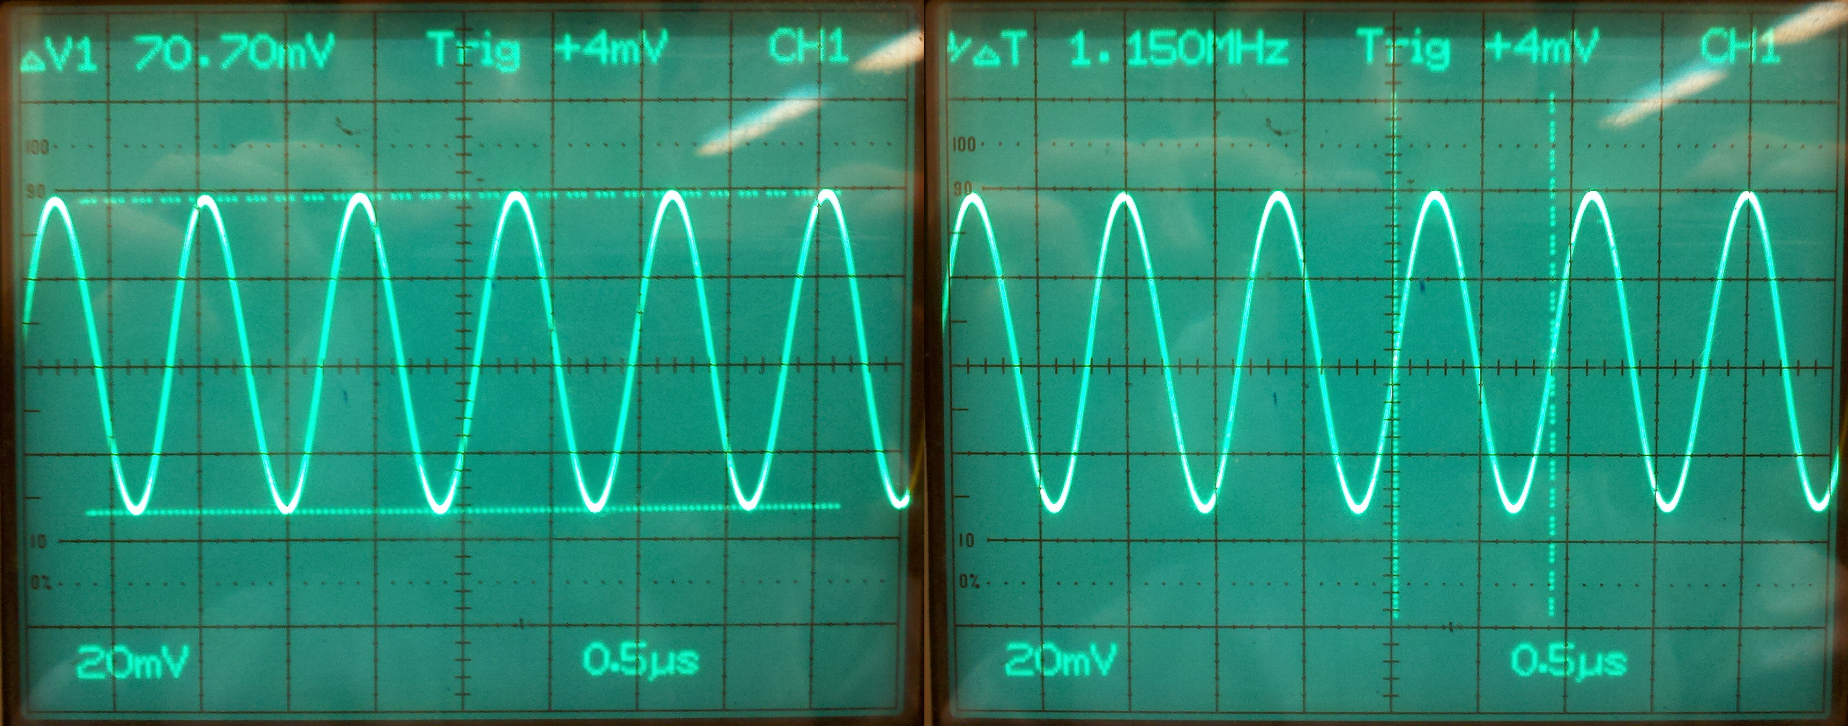
\includegraphics[width=\linewidth, keepaspectratio=true]{lab1_images/10x_sine_corner.png} 
	\caption{Oscilloscope reading at corner frequency (1.15 MHz) for 10x probe in series with a 10k resistor. }
	\label{fig:probe_corner}
\end{figure}

Figure \ref{fig:bnc_circuit} shows the model used for the BNC circuit (a low pass filter), and Figure \ref{fig:bnc_corner} shows the oscilloscope reading at the corner frequency (135 kHz). Similarly, Figure \ref{fig:probe_circuit} shows the model for the 10x probe circuit, and Figure \ref{fig:probe_corner} shows the scope reading at the corner frequency (1.15 MHz).

\subsection*{Simulated Results}

\begin{figure}
	\centering
	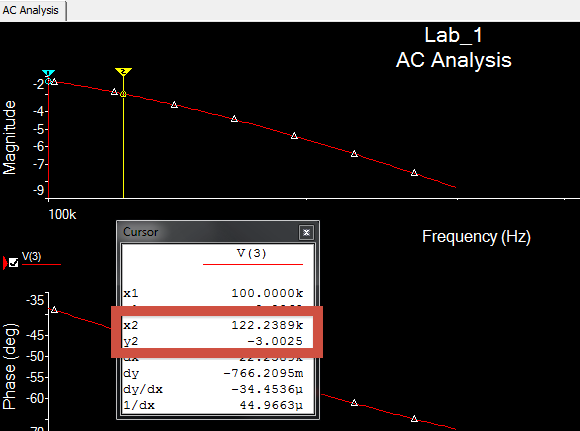
\includegraphics[width=\figwidth, keepaspectratio=true]{lab1_images/BNC_bode.png} 
	\caption{Multisim created Bode Plot for the BNC circuit. The information box summarizes the onscreen marker - y2 is in dB and x2 is in Hz. }
	\label{fig:bnc_bode}
\end{figure}

\begin{figure}
	\centering
	\includegraphics[width=\figwidth, keepaspectratio=true]{lab1_images/10x_bode.png} 
	\caption{Multisim created Bode Plot for the 10x probe circuit. The information box summarizes the onscreen marker - y2 is in dB and x2 is in Hz. }
	\label{fig:probe_bode}
\end{figure}

Figures \ref{fig:bnc_bode} and \ref{fig:probe_bode} show the bode plots, produced by MultiSim, for the BNC circuit and the 10x scope circuit respectively. Figures \ref{fig:bnc_circuit} and \ref{fig:probe_circuit} show the MultiSim circuits which correspond to these bode plots. Table \ref{table:corners} summarizes the expected and measured corner frequencies for the two circuits.

\begin{center}
\begin{table}[ht]
\caption{Corner Frequencies (expected and estimated)}
\centering 
	\begin{tabular}{| c | c | c |}
	\hline
	& \textbf{BNC/Coax} & \textbf{10X Probe} \\
	\hline
	\textbf{Expected} & 122 kHz & 1.09 MHz \\
	\textbf{Measured} & 135 kHz & 1.15 MHz \\
	\hline
	\end{tabular}
	\label{table:corners}
\end{table}
\end{center}

The measured corner frequencies for the BNC and 10x probe circuits are 10\% and 6\% greater than expected respectively. These differences can be partially attributed to the fact that our model does not take the connecting cable between the function generator and bread board into account, which has a non-neglible capacitance. Similarly, the BNC splitters used to connect components of the circuit also have a non-zero capacitance that would affect the measured corner frequency.

\subsection*{Fourier Analysis}

\begin{figure}
	\centering
	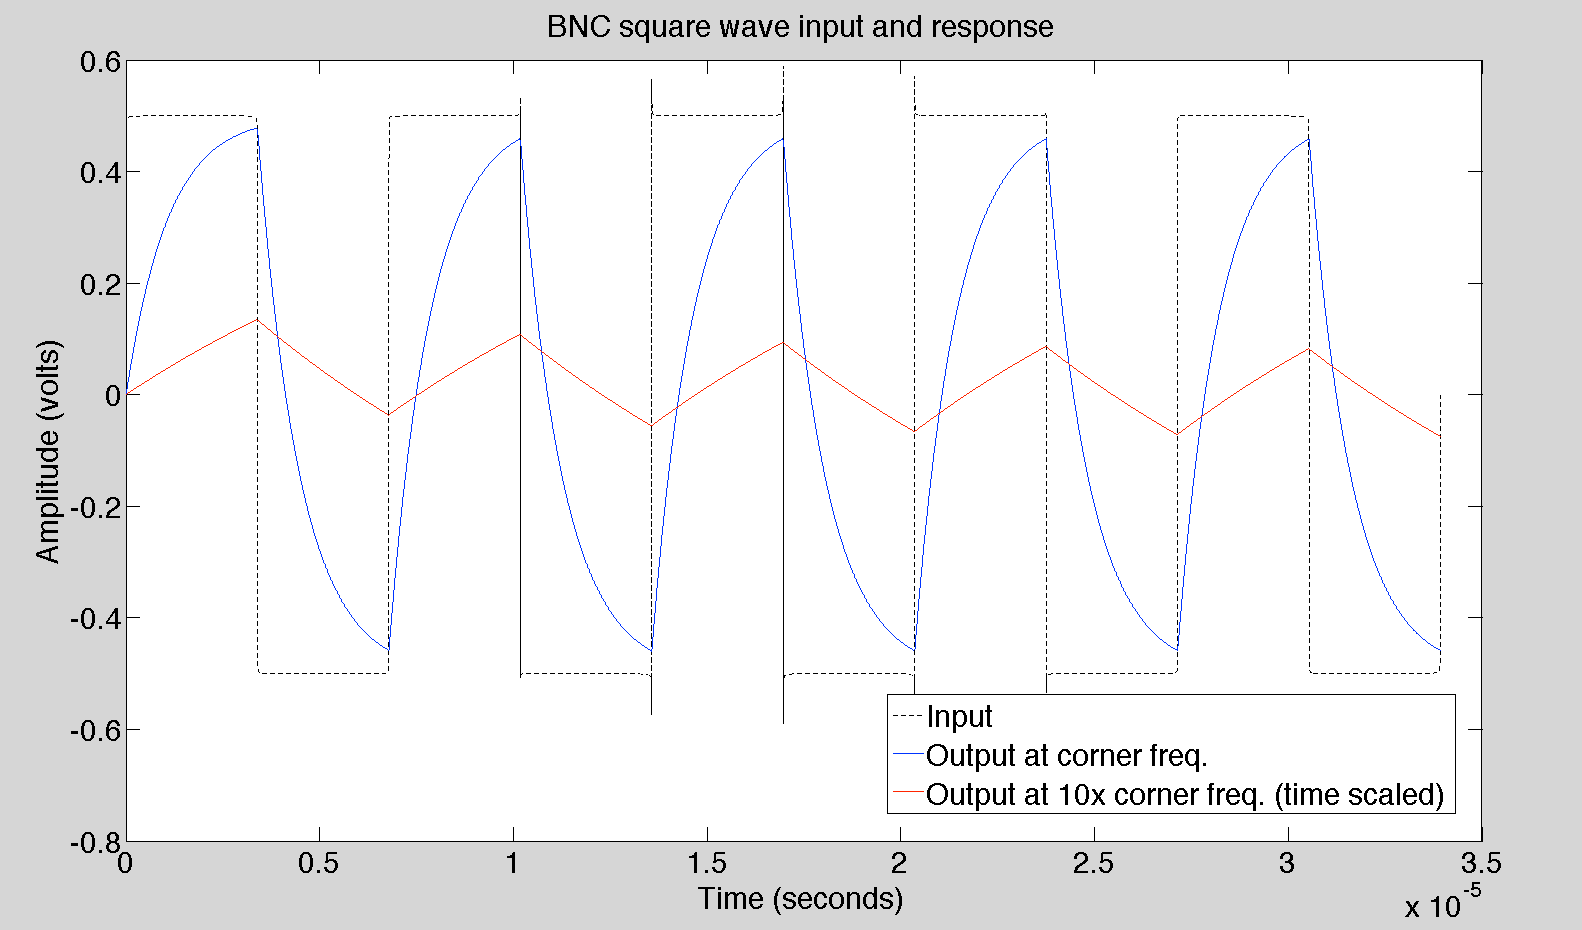
\includegraphics[width=\linewidth, keepaspectratio=true]{lab1_images/MATLAB_BNC_square.png} 
	\caption{BNC circuit's simulated response to a square wave at the corner frequency and 10 times the corner frequency.}
	\label{fig:bnc_square}
\end{figure}

\begin{figure}
	\centering
	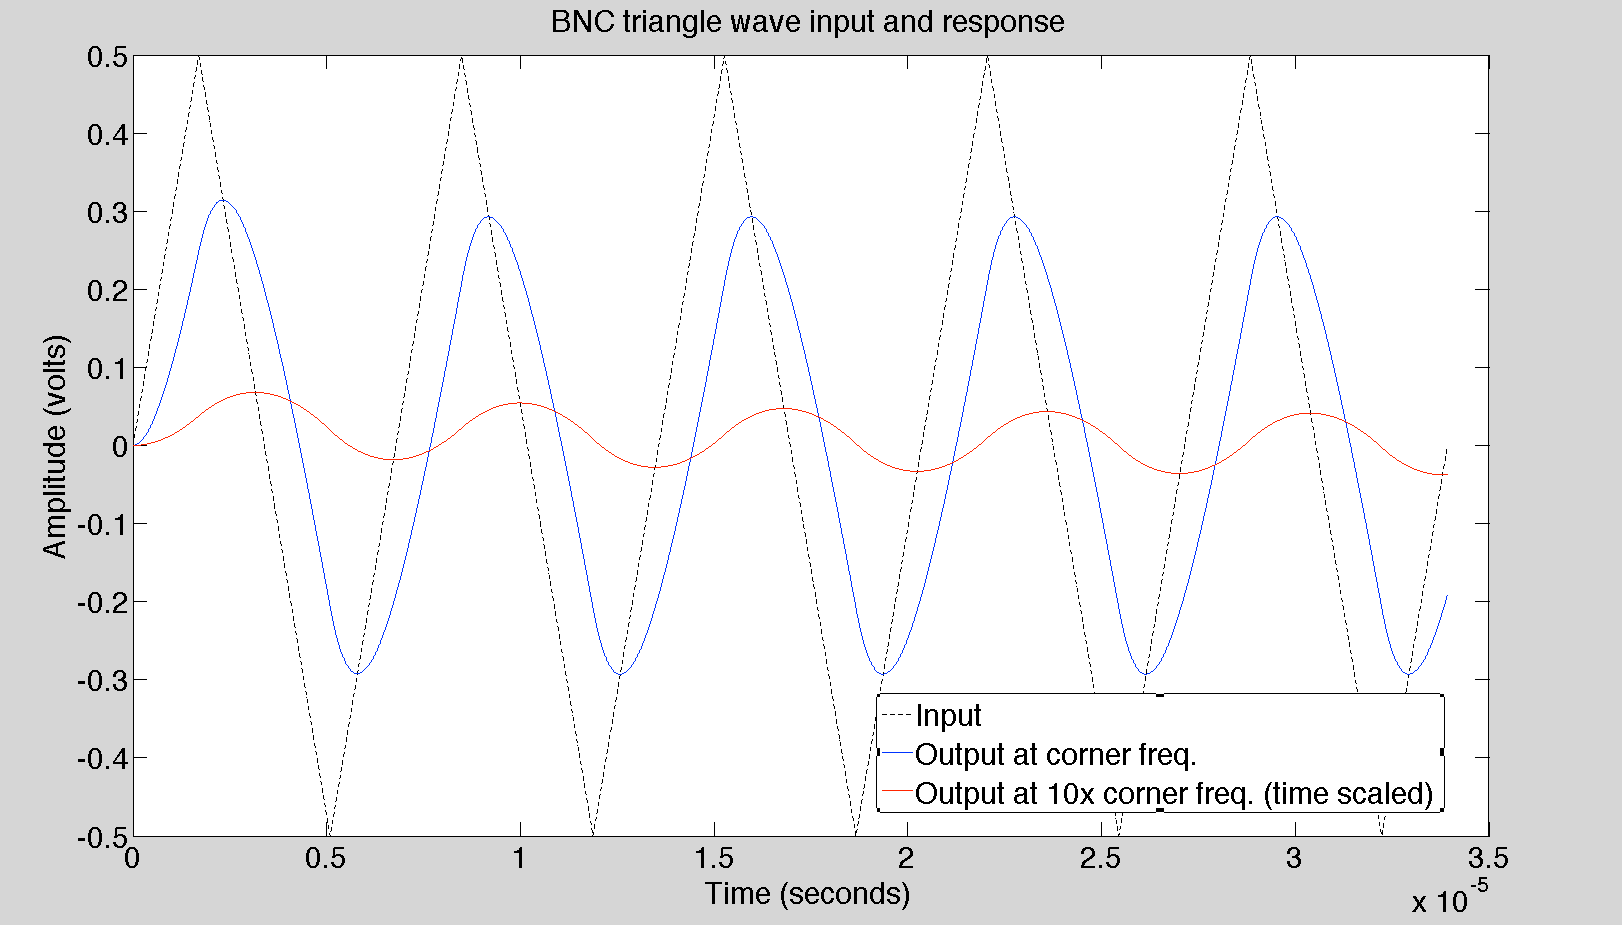
\includegraphics[width=\linewidth, keepaspectratio=true]{lab1_images/MATLAB_BNC_triangle.png} 
	\caption{BNC circuit's simulated response to a square wave at the corner frequency and 10 times the corner frequency.}
	\label{fig:bnc_triangle}
\end{figure}

\begin{figure}
	\centering
	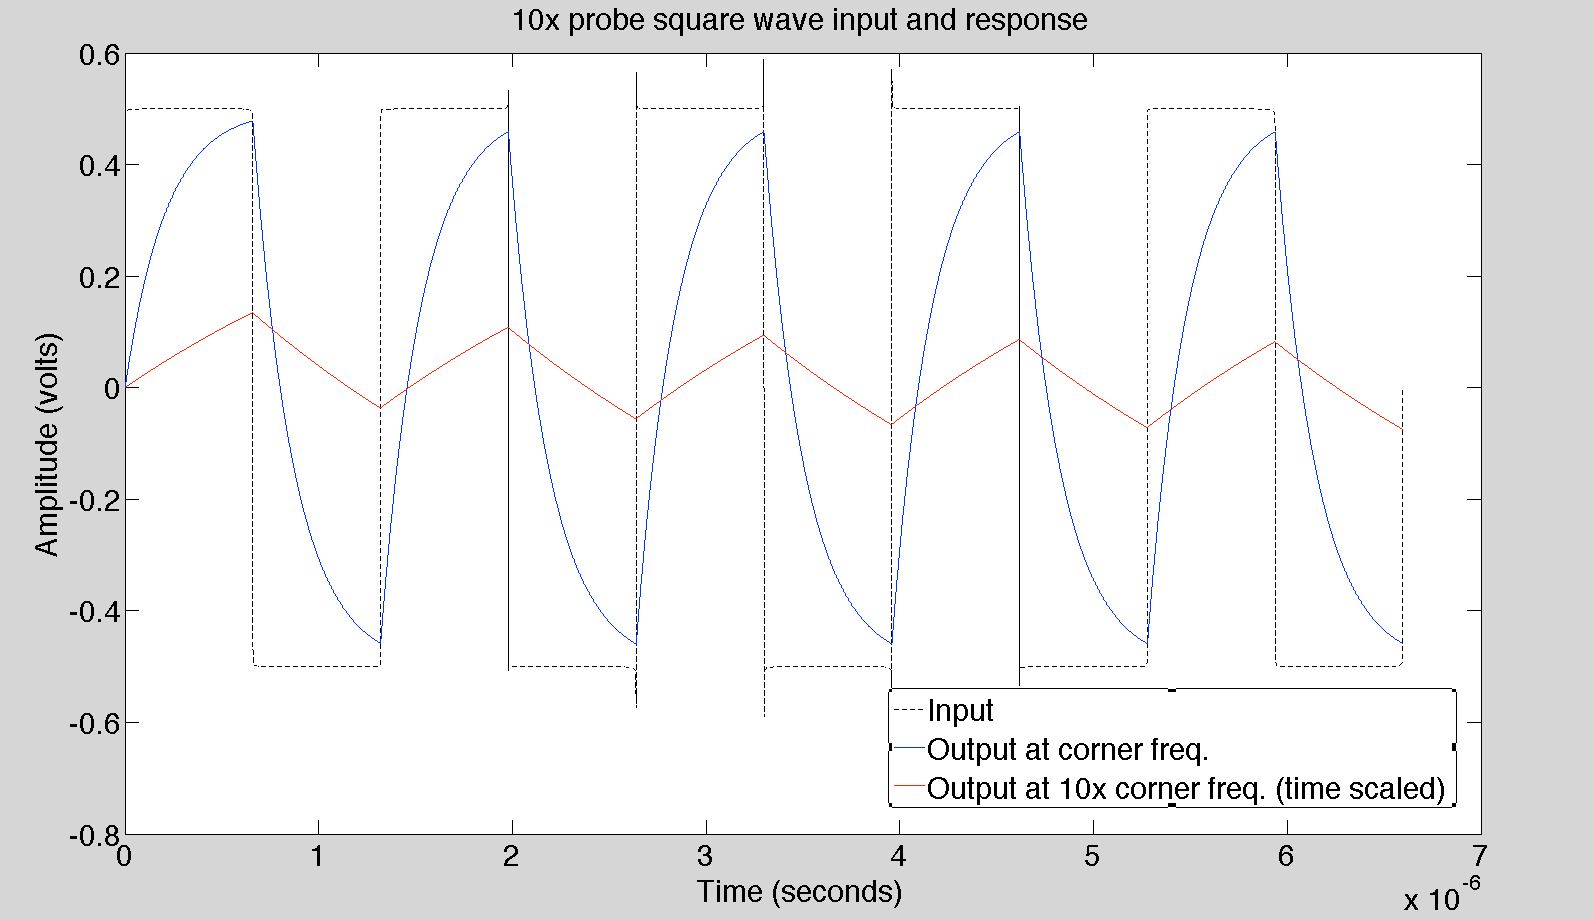
\includegraphics[width=\linewidth, keepaspectratio=true]{lab1_images/MATLAB_10x_square.png} 
	\caption{10x probe circuit's simulated response to a square wave at the corner frequency and 10 times the corner frequency.}
	\label{fig:probe_square}
\end{figure}

\begin{figure}
	\centering
	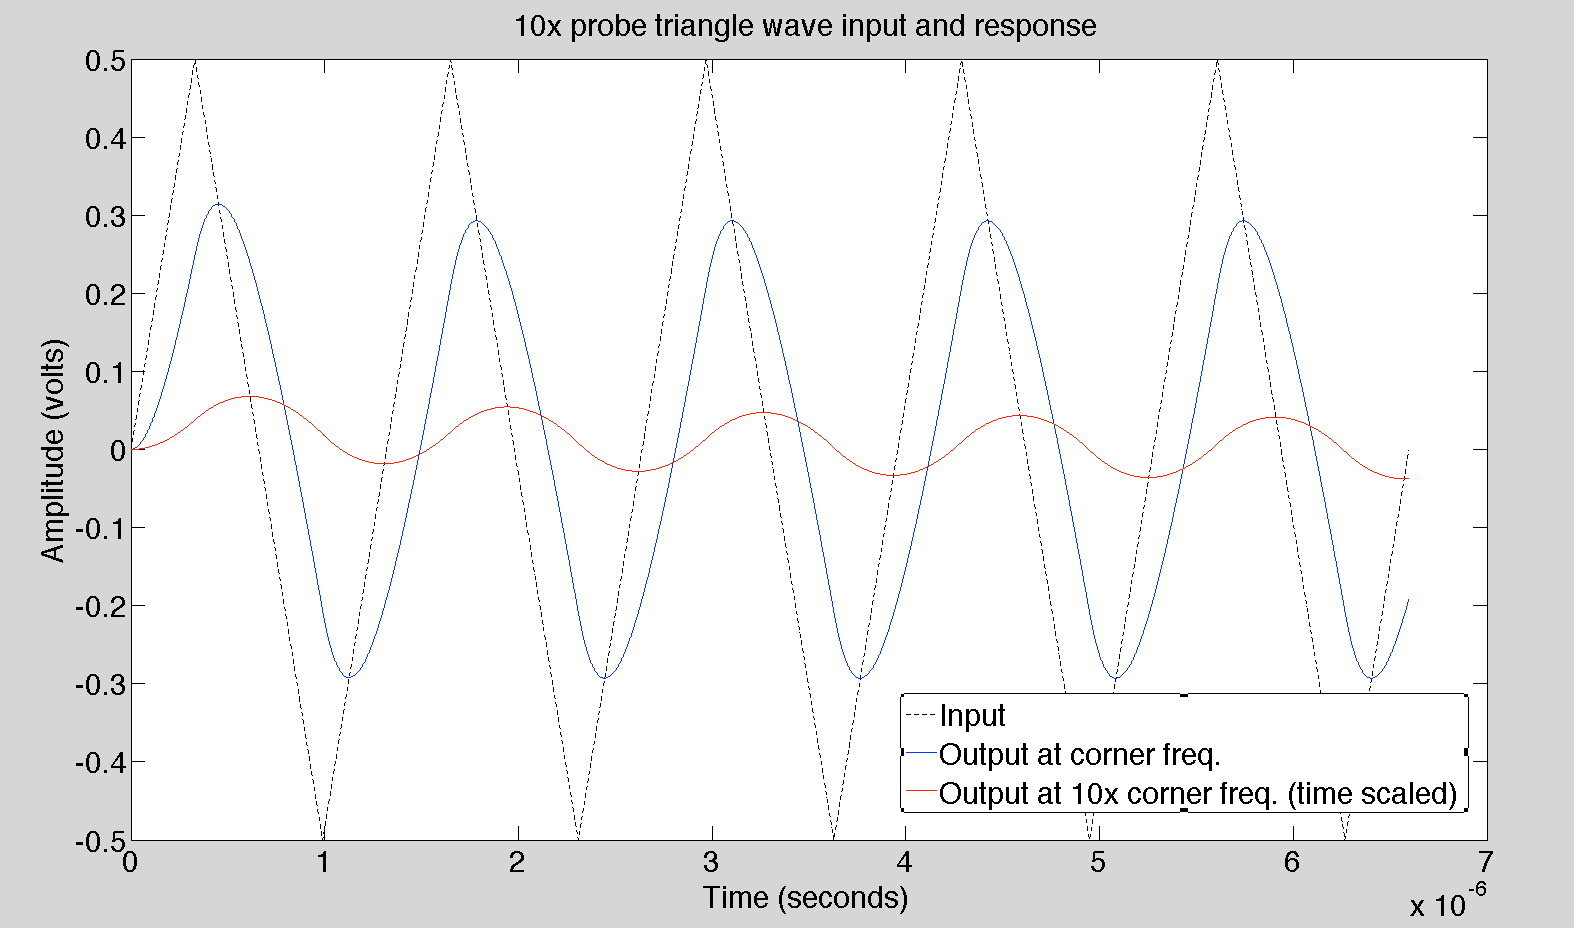
\includegraphics[width=\linewidth, keepaspectratio=true]{lab1_images/MATLAB_10x_triangle.png} 
	\caption{10x probe circuit's simulated response to a square wave at the corner frequency and 10 times the corner frequency.}
	\label{fig:probe_triangle}
\end{figure}

Figures \ref{fig:bnc_square}, \ref{fig:bnc_triangle}, \ref{fig:probe_square}, and \ref{fig:probe_triangle} show the results of a MATLAB-aided analysis of square and triangle wave inputs into both systems at the corner frequency and 10 times the corner frequency. The analysis used the MATLAB transfer function construct alongside its linear simulation tool with inputs built from the Fourier Series of square and triangle waves. The inputs at 10x the corner frequencies are time scaled by 10 so they match up on the same time axis as the input. Note that since the analysis models both systems as a first order low pass filter, the two pairs of plots (one for BNC and one for the 10x probe) are exactly the same just on a different time scale.

\section*{Section C: Appendix}
\subsection*{MATLAB Code}
\begin{verbatim}
%% Analysis based on input capacitance
Cin_probe = 21e-12; % 21 pF
square_and_triangle_analysis(Cin_probe, '10x probe')

Cin_bnc = 108e-12; % 108 pF
square_and_triangle_analysis(Cin_bnc, 'BNC')


function square_and_triangle_analysis( input_capacitance, label )
%square_and_triangle_analysis Function to analyze what a square and 
% triangle wave looks like at the corner and 10x corner frequency.
%   We are modeling the response of a capacitor in series with
%   a function generator having a 10 kOhm source impedance. This is a first
%   order low pass filter and is a simplistic model of a 10x probe and a
%   BNC cable (each one having a different input capacitance.)

R = 10e3; % 10 kOhm

tau = R * input_capacitance;
wc = 1/tau;
fc = wc/(2*pi);

H = tf(1, [tau 1]);

% fourier series harmonics we'll use to create a square and triangle wave
harmonics = (1:1:999)'; 

%% corner frequency
t_fc = linspace(0,5/fc,10000); % 5 periods of the waves
square = square_wave(t_fc, 0.5, fc, harmonics,...
    ones(length(harmonics),1));
triangle = triangle_wave(t_fc, 0.5, fc, harmonics,...
    ones(length(harmonics),1));

[y_square_fc, t_fc] = lsim(H,square,t_fc);
[y_triangle_fc, t_fc] = lsim(H,triangle,t_fc);


%% 10x corner frequency
t_10fc = linspace(0,5/(10*fc),10000);
square = square_wave(t_10fc, 0.5, 10*fc, harmonics, ...
    ones(length(harmonics),1));
triangle = triangle_wave(t_10fc, 0.5, 10*fc, harmonics, ...
    ones(length(harmonics),1));

[y_square_10fc, t_10fc] = lsim(H,square,t_10fc);
[y_triangle_10fc, t_10fc] = lsim(H,triangle,t_10fc);


%% Plotting

figure
plot(t_fc, square, 'k--')
hold on
plot(t_fc, y_square_fc, 'b')
hold on
plot(10*t_10fc, y_square_10fc,'r')
title(strcat(label, ' square wave input and response'),'FontSize',30)
ylabel('Amplitude (volts)','FontSize',30)
xlabel('Time (seconds)','FontSize',30)
legend('Input','Output at corner freq.',...
    'Output at 10x corner freq. (time scaled)')
set(gca,'FontSize',30)

figure
plot(t_fc, triangle, 'k--')
hold on
plot(t_fc, y_triangle_fc, 'b')
hold on
plot(10*t_10fc, y_triangle_10fc,'r')
title(strcat(label, ' triangle wave input and response'),'FontSize',30)
ylabel('Amplitude (volts)','FontSize',30)
xlabel('Time (seconds)','FontSize',30)
legend('Input','Output at corner freq.',...
    'Output at 10x corner freq. (time scaled)')
set(gca,'FontSize',30)

end


function [ square ] = square_wave( t_in, A, f, harmonics, gains )
%SQUARE_WAVE Produces a square wave of specified parameters
%   Produces a square wave using the fourier series with as many harmonics
%   as specified in the harmonics input. harmonics and gains are both
%   vectors (of the same length) representing what harmonics are present
%   and the gain for each harmonic. A is the amplitude, f is the freq.

square_fun = @(t, n) A * (4/pi) * gains(n) .* ...
                        (sin(2*pi*(2*n - 1)*f*t) ./ (2*n - 1));

square = sum(bsxfun(square_fun, t_in, harmonics), 1)';

end


function [ triangle ] = triangle_wave( t, A, f, harmonics, gains )
%TRIANGLE_WAVE Produces a triangle wave of specified parameters
%   Produces a triangle wave using the fourier series with as many harmonics
%   as specified in the harmonics input. harmonics and gains are both
%   vectors (of the same length) representing what harmonics are present
%   and the gain for each harmonic. A is the amplitude, f is the freq.

triangle_fun = @(t, n) A * (8/pi^2) * gains(n) .* (-1).^(n-1) .* ...
                            (sin(2*pi*(2*n - 1)*f*t) ./ (2*n - 1).^2);

triangle = sum(bsxfun(triangle_fun, t, harmonics), 1)';

end
\end{verbatim}
\end{document}